\documentclass{article}
\usepackage[T1]{fontenc}
\usepackage{lmodern}
\usepackage{graphicx}
\usepackage{amsmath,amssymb}
\usepackage[a4paper,margin=2cm]{geometry}
\usepackage[absolute,overlay]{textpos}
\setlength{\TPHorizModule}{1mm}
\setlength{\TPVertModule}{1mm}
\usepackage[indonesian]{babel}
\usepackage{hyperref}
\setlength{\emergencystretch}{2em}
% unit: Halaman 17

\begin{document}

% === Halaman 17 (python/native) ===

Permutasi Awal

• Tujuan: mengacak plainteks sehingga urutan bit-bit 

   di dalamnya berubah. 

• Matriks permutasi awal (IP):


58 

50 

42 

34 

26 

18 

10 

2 

60 

52 

44 

36 

28 

20 

12 

4 

62 

54 

46 

38 

30 

22 

14 

6 

64 

56 

48 

40 

32 

24 

16 

8 

57 

49 

41 

33 

25 

17 

9 

1 

59 

51 

43 

35 

27 

19 

11 

3 

61 

53 

45 

37 

29 

21 

13 

5 

63 

55 

47 

39 

31 

23 

15 

7 


17

% deskripsi: gambar native xref 38
\noindent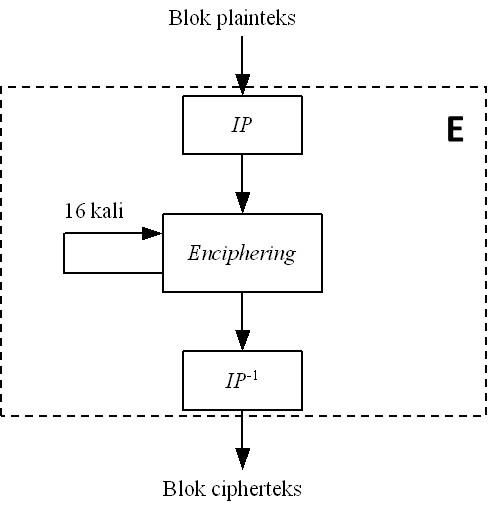
\includegraphics[width=0.85\textwidth]{../../images/python/page_017_img_01.jpeg}

\end{document}
